% =====================================================================
% IBFE Tutorials: classical immersed boundary formulation
% =====================================================================
\documentclass[aspectratio=169,11pt]{beamer}

% Match the visual language of the SIAM Waves talk.
\usetheme{Boadilla}
\usecolortheme{seahorse}
\useinnertheme{rectangles}
\useoutertheme{infolines}

\setbeamercolor{structure}{fg=blue!55!black}
\setbeamercolor{title}{fg=white,bg=blue!55!black}
\setbeamercolor{frametitle}{fg=blue!55!black}
\setbeamercolor{block title}{bg=blue!12,fg=blue!55!black}
\setbeamercolor{block body}{bg=blue!4}
\setbeamertemplate{navigation symbols}{}
\setbeamerfont{frametitle}{series=\bfseries,size=\large}
\setbeamerfont{title}{series=\bfseries,size=\Large}

\usepackage[T1]{fontenc}
\usepackage[utf8]{inputenc}
\DeclareFontShape{T1}{cmss}{b}{n}{<->ssub*cmss/bx/n}{}
\usepackage{graphicx}
\graphicspath{{./}{../}}
\usepackage{amsmath,amssymb,bm,mathtools}
\usepackage{booktabs}
\usepackage{xcolor}
\usepackage{tcolorbox}
\tcbuselibrary{skins}
\usepackage{tikz}
\usetikzlibrary{arrows.meta}
\usepackage{hyperref}
\hypersetup{colorlinks=true,urlcolor=blue!55!black}

\newcommand{\hi}[1]{\textcolor{blue!55!black}{\textbf{#1}}}
\newcommand{\warn}[1]{\textcolor{red!70!black}{\textbf{#1}}}
\newcommand{\soft}[1]{\textcolor{gray!50!black}{#1}}
\newcommand{\uvec}{\bm{u}}
\newcommand{\xvec}{\bm{x}}
\newcommand{\Xvec}{\bm{X}}
\newcommand{\Uvec}{\bm{U}}
\newcommand{\fvec}{\bm{f}}
\newcommand{\Fvec}{\bm{F}}
\newcommand{\Yvec}{\bm{Y}}
\newcommand{\etavec}{\bm{\eta}}
\newcommand{\ivec}{\bm{i}}

\newtcolorbox{punchbox}{
  enhanced,
  colback=blue!4,
  colframe=blue!55!black,
  boxrule=0.6pt,
  arc=2pt,
  left=4pt,right=4pt,top=3pt,bottom=3pt
}

\title[Classical IB formulation]{The classical immersed boundary method}
\subtitle{Mathematical formulation and numerical considerations}
\author[Miller]{Laura A. Miller}
\institute[UArizona]{Department of Mathematics, University of Arizona}
\date{}

\begin{document}

% ----- 1. Title -----
\begin{frame}[plain]
  \begin{beamercolorbox}[sep=10pt,center]{title}
    {\bfseries\Large The classical immersed boundary method}\\[3pt]
    {\normalsize Mathematical formulation and numerical considerations}
  \end{beamercolorbox}
  \vspace{1.3em}
  \begin{columns}[T,onlytextwidth]
  \begin{column}{0.55\textwidth}
    \textbf{\large Laura A. Miller}\\[4pt]
    Department of Mathematics\\
    University of Arizona\\[14pt]
    {\small IBFE Tutorials}
  \end{column}
  \begin{column}{0.45\textwidth}
    \begin{punchbox}
    \centering
    Eulerian fluid\\[2pt]
    \(\uvec(\xvec,t),\ p(\xvec,t),\ \fvec(\xvec,t)\)\\[8pt]
    Lagrangian structure\\[2pt]
    \(\Xvec(q,t),\ \Uvec(q,t),\ \Fvec(q,t)\)
    \end{punchbox}
  \end{column}
  \end{columns}
  \vfill
  \centering{\tiny\color{black!55}AI tools were used to assist with formatting, organization, and clarification of the instructor's original notes.}
\end{frame}

\section{Fluid--structure interaction}

% ----- 2. Biological regimes -----
\begin{frame}{Fluid--structure interaction spans many scales}
\begin{columns}[T,onlytextwidth]
\begin{column}{0.32\textwidth}
\textbf{Higher Reynolds number}
\begin{itemize}\itemsep5pt
  \item whale heart: chambered pumping
  \item stingray: flapping locomotion
\end{itemize}
\medskip
\textbf{Lower Reynolds number}
\begin{itemize}\itemsep5pt
  \item respiratory cilia: microscopic pumping
  \item \emph{E. coli}: flagellar locomotion
\end{itemize}
\end{column}
\begin{column}{0.68\textwidth}
\centering
\resizebox{\linewidth}{!}{%
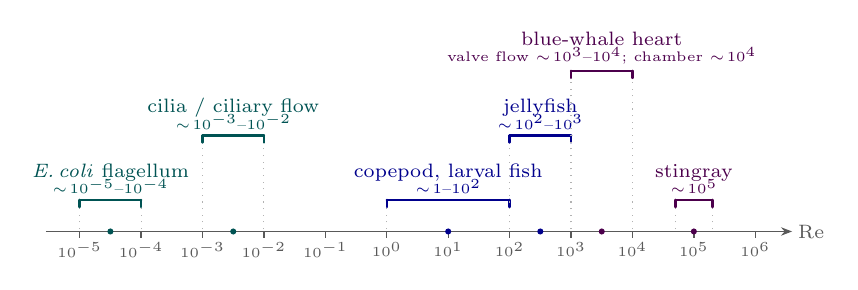
\begin{tikzpicture}[
  x=0.78cm, y=1cm, font=\scriptsize,
  brk/.style={line width=0.9pt,line cap=round},
  lead/.style={draw=black!30,dotted,line width=0.4pt}
]
% --- logarithmic Re axis -------------------------------------------------
\draw[-{Stealth[length=4pt]},line width=0.7pt,black!65] (-5.55,0) -- (6.6,0);
\node[anchor=west,black!65,inner sep=2pt] at (6.6,0) {$\mathrm{Re}$};
\foreach \e in {-5,-4,-3,-2,-1,0,1,2,3,4,5,6}{%
  \draw[black!65,line width=0.5pt] (\e,0) -- (\e,-0.08);
  \node[anchor=north,font=\tiny,black!65,inner sep=1.5pt] at (\e,-0.08) {$10^{\e}$};
}
% --- viscous end: bacterial flagellum ------------------------------------
\draw[lead] (-5,0.03) -- (-5,0.40);  \draw[lead] (-4,0.03) -- (-4,0.40);
\draw[teal!65!black,brk] (-5,0.40) -- (-4,0.40);
\draw[teal!65!black,brk] (-5,0.40) -- (-5,0.31);
\draw[teal!65!black,brk] (-4,0.40) -- (-4,0.31);
\fill[teal!65!black] (-4.5,0) circle (1.1pt);
\node[anchor=south,align=center,text=teal!65!black,inner sep=1.5pt] at (-4.5,0.42)
  {\emph{E.\,coli} flagellum\\[-2pt]{\tiny $\sim\!10^{-5}$--$10^{-4}$}};
% --- cilia ---------------------------------------------------------------
\draw[lead] (-3,0.03) -- (-3,1.22);  \draw[lead] (-2,0.03) -- (-2,1.22);
\draw[teal!65!black,brk] (-3,1.22) -- (-2,1.22);
\draw[teal!65!black,brk] (-3,1.22) -- (-3,1.13);
\draw[teal!65!black,brk] (-2,1.22) -- (-2,1.13);
\fill[teal!65!black] (-2.5,0) circle (1.1pt);
\node[anchor=south,align=center,text=teal!65!black,inner sep=1.5pt] at (-2.5,1.24)
  {cilia / ciliary flow\\[-2pt]{\tiny $\sim\!10^{-3}$--$10^{-2}$}};
% --- copepods and larval fish -------------------------------------------
\draw[lead] (0,0.03) -- (0,0.40);  \draw[lead] (2,0.03) -- (2,0.40);
\draw[blue!55!black,brk] (0,0.40) -- (2,0.40);
\draw[blue!55!black,brk] (0,0.40) -- (0,0.31);
\draw[blue!55!black,brk] (2,0.40) -- (2,0.31);
\fill[blue!55!black] (1,0) circle (1.1pt);
\node[anchor=south,align=center,text=blue!55!black,inner sep=1.5pt] at (1,0.42)
  {copepod, larval fish\\[-2pt]{\tiny $\sim\!1$--$10^{2}$}};
% --- jellyfish -----------------------------------------------------------
\draw[lead] (2,0.03) -- (2,1.22);  \draw[lead] (3,0.03) -- (3,1.22);
\draw[blue!55!black,brk] (2,1.22) -- (3,1.22);
\draw[blue!55!black,brk] (2,1.22) -- (2,1.13);
\draw[blue!55!black,brk] (3,1.22) -- (3,1.13);
\fill[blue!55!black] (2.5,0) circle (1.1pt);
\node[anchor=south,align=center,text=blue!55!black,inner sep=1.5pt] at (2.5,1.24)
  {jellyfish\\[-2pt]{\tiny $\sim\!10^{2}$--$10^{3}$}};
% --- blue-whale heart ----------------------------------------------------
\draw[lead] (3,0.03) -- (3,2.04);  \draw[lead] (4,0.03) -- (4,2.04);
\draw[violet!60!black,brk] (3,2.04) -- (4,2.04);
\draw[violet!60!black,brk] (3,2.04) -- (3,1.95);
\draw[violet!60!black,brk] (4,2.04) -- (4,1.95);
\fill[violet!60!black] (3.5,0) circle (1.1pt);
\node[anchor=south,align=center,text=violet!60!black,inner sep=1.5pt] at (3.5,2.06)
  {blue-whale heart\\[-2pt]{\tiny valve flow $\sim\!10^{3}$--$10^{4}$; chamber $\sim\!10^{4}$}};
% --- stingray ------------------------------------------------------------
\draw[lead] (4.7,0.03) -- (4.7,0.40);  \draw[lead] (5.3,0.03) -- (5.3,0.40);
\draw[violet!60!black,brk] (4.7,0.40) -- (5.3,0.40);
\draw[violet!60!black,brk] (4.7,0.40) -- (4.7,0.31);
\draw[violet!60!black,brk] (5.3,0.40) -- (5.3,0.31);
\fill[violet!60!black] (5,0) circle (1.1pt);
\node[anchor=south,align=center,text=violet!60!black,inner sep=1.5pt] at (5,0.42)
  {stingray\\[-2pt]{\tiny $\sim\!10^{5}$}};
\end{tikzpicture}}\\[2pt]
{\scriptsize Schematic: orders of magnitude, instructor's course notes.}
\end{column}
\end{columns}
\begin{punchbox}
\small The same conservation laws apply across these examples; the Reynolds number identifies the balance between inertia and viscosity.
\end{punchbox}
\end{frame}

% ----- 3. Dimensional fluid equations -----
\begin{frame}{Modeling the fluid: incompressible Navier--Stokes}
Let \(\uvec(\xvec,t)\) be velocity and \(p(\xvec,t)\) pressure. For constant density \(\rho\) and dynamic viscosity \(\mu\),
\[
  \rho\left(
  \frac{\partial\uvec}{\partial t}
  +(\uvec\cdot\nabla)\uvec
  \right)
  =
  -\nabla p+\mu\Delta\uvec+\fvec,
  \qquad
  \nabla\cdot\uvec=0.
\]
\begin{columns}[T,onlytextwidth]
\begin{column}{0.49\textwidth}
\textbf{Momentum balance}
\begin{itemize}\itemsep5pt
  \item local and advective acceleration
  \item pressure and viscous forces
  \item immersed-structure force \(\fvec\)
\end{itemize}
\end{column}
\begin{column}{0.49\textwidth}
\textbf{Incompressibility}
\begin{itemize}\itemsep5pt
  \item velocity is divergence free
  \item pressure enforces the constraint
  \item density is transported as a constant
\end{itemize}
\end{column}
\end{columns}
\end{frame}

% ----- 4. Nondimensional form -----
\begin{frame}{Nondimensional Navier--Stokes equations}
Choose characteristic length \(L\) and speed \(U\):
\[
  \xvec=L\xvec^*,
  \qquad
  t=\frac{L}{U}t^*,
  \qquad
  \uvec=U\uvec^*,
  \qquad
  p=\rho U^2p^*.
\]
With \(\fvec=(\rho U^2/L)\fvec^*\),
\[
  \frac{\partial\uvec^*}{\partial t^*}
  +(\uvec^*\cdot\nabla^*)\uvec^*
  =
  -\nabla^*p^*
  +\frac{1}{\mathrm{Re}}\Delta^*\uvec^*
  +\fvec^*,
  \qquad
  \nabla^*\cdot\uvec^*=0,
\]
\[
  \boxed{\mathrm{Re}=\frac{\rho UL}{\mu}=\frac{UL}{\nu}},
  \qquad \nu=\frac{\mu}{\rho}.
\]
\end{frame}

% ----- 5. Reynolds number -----
\begin{frame}{Reynolds number and dynamic similarity}
\begin{columns}[T,onlytextwidth]
\begin{column}{0.52\textwidth}
\[
  \mathrm{Re}
  =
  \frac{\text{inertial scale}}{\text{viscous scale}}
  =
  \frac{\rho UL}{\mu}.
\]
\begin{itemize}\itemsep6pt
  \item \(\mathrm{Re}\ll1\): viscosity dominates.
  \item \(\mathrm{Re}\gg1\): inertia is important.
  \item Changing size, speed, density, or viscosity changes the regime.
\end{itemize}
\end{column}
\begin{column}{0.48\textwidth}
\begin{punchbox}
\textbf{Similarity needs more than one number.}\\[3pt]
Matching \(\mathrm{Re}\) supports dynamic similarity only when the nondimensional geometry, boundary motion, constitutive laws, and other relevant parameters also match.
\end{punchbox}
\end{column}
\end{columns}
\end{frame}

% ----- 6. Boundary model -----
\begin{frame}{Describing the immersed boundary}
\begin{columns}[T,onlytextwidth]
\begin{column}{0.52\textwidth}
\textbf{Classical interfacial model}
\begin{itemize}\itemsep6pt
  \item A material coordinate \(q\in\mathcal U\subset\mathbb R\) labels a massless curve.
  \item \(\Gamma_t=\Xvec(\mathcal U,t)\) is its current position.
  \item Elastic energy may resist stretching or bending.
  \item Constitutive parameters may vary in space or time.
\end{itemize}
\end{column}
\begin{column}{0.48\textwidth}
\textbf{Rigid or prescribed motion}
\begin{itemize}\itemsep6pt
  \item Stiff elasticity can approximate rigidity, but creates a stiff numerical problem.
  \item Target-point penalties impose motion approximately.
  \item Exact constraints require unknown reaction forces.
\end{itemize}
\begin{punchbox}
\small Immersed boundaries are represented through forces; they need not describe a passive elastic material.
\end{punchbox}
\end{column}
\end{columns}
\end{frame}

% ----- 7. Two descriptions -----
\begin{frame}{Eulerian fluid, Lagrangian structure}
\begin{columns}[T,onlytextwidth]
\begin{column}{0.49\textwidth}
\begin{block}{Eulerian description}
The fixed Cartesian grid carries
\[
  \uvec(\xvec,t),\qquad p(\xvec,t),\qquad \fvec(\xvec,t).
\]
The fluid equations are solved at spatial locations \(\xvec\in\Omega\).
\end{block}
\end{column}
\begin{column}{0.49\textwidth}
\begin{block}{Lagrangian description}
The moving curvilinear mesh carries
\[
  \Xvec(q,t),\qquad \Uvec(q,t),\qquad \Fvec(q,t).
\]
The material label \(q\) follows the structure.
\end{block}
\end{column}
\end{columns}
\begin{punchbox}
\centering
\(\Fvec\overset{\text{spread}}{\longrightarrow}\fvec\),
\qquad
\(\uvec\overset{\text{interpolate}}{\longrightarrow}\Uvec=\partial_t\Xvec\).
The grids do not conform to one another.
\end{punchbox}
\end{frame}

\section{Continuum formulation}

% ----- 8. Complete system -----
\begin{frame}{The governing coupling equations}
\small
\begin{align*}
\rho\left(\frac{\partial\uvec}{\partial t}+(\uvec\cdot\nabla)\uvec\right)
  &= -\nabla p+\mu\Delta\uvec+\fvec,
  & \nabla\cdot\uvec&=0,\\[2pt]
\fvec(\xvec,t)
  &=\int_{\mathcal U}\Fvec(q,t)
  \delta^{(2)}\!\left(\xvec-\Xvec(q,t)\right)\,dq,\\[2pt]
\frac{\partial\Xvec}{\partial t}(q,t)=\Uvec(q,t)
  &=\int_{\Omega}\uvec(\xvec,t)
  \delta^{(2)}\!\left(\xvec-\Xvec(q,t)\right)\,d\xvec,\\[2pt]
\Fvec(q,t)&=-\frac{\delta E[\Xvec,t]}{\delta\Xvec}(q,t).
\end{align*}
\begin{punchbox}
\centering
These equations require compatible initial data and fluid boundary conditions. The scope here is a two-dimensional, massless elastic curve with no slip.
\end{punchbox}
\soft{\scriptsize Sources: Peskin (2002); Griffith and Patankar (2020).}
\end{frame}

% ----- 9. Elastic energy -----
\begin{frame}{Elastic energy determines the force}
The variational definition fixes the sign:
\[
  \delta E[\Xvec,t;\etavec]
  =
  -\int_{\mathcal U}\Fvec(q,t)\cdot\etavec(q)\,dq,
  \qquad
  \boxed{\Fvec=-\frac{\delta E}{\delta\Xvec}}.
\]
\begin{columns}[T,onlytextwidth]
\begin{column}{0.51\textwidth}
\textbf{Typical contributions}
\begin{itemize}\itemsep6pt
  \item stretching: depends on \(\lvert\partial_q\Xvec\rvert\)
  \item bending: depends on curvature
  \item active terms: prescribe a preferred configuration or tension
\end{itemize}
\end{column}
\begin{column}{0.49\textwidth}
\begin{punchbox}
\small \(\Fvec(q,t)\,dq\) is the force that material segment \(dq\) applies to the fluid. Explicit time dependence permits prescribed changes in the constitutive model.
\end{punchbox}
\end{column}
\end{columns}
\end{frame}

% ----- 10. Target points -----
\begin{frame}{Target points impose motion approximately}
Let \(\Yvec(q,t)\) be the desired trajectory while \(\Xvec(q,t)\) still moves with the fluid:
\[
  E_{\mathrm{target}}[\Xvec,t]
  =
  \frac{\kappa}{2}
  \int_{\mathcal U}
  \lvert\Xvec(q,t)-\Yvec(q,t)\rvert^2\,dq,
  \qquad
  \Fvec_{\mathrm{target}}=\kappa(\Yvec-\Xvec).
\]
\begin{itemize}\itemsep6pt
  \item Finite \(\kappa\) allows displacement error.
  \item Damping may also penalize the velocity mismatch.
  \item Increasing \(\kappa\) can reduce tracking error only while the discretization remains stable and resolved.
  \item An exact prescribed-motion constraint instead solves for a Lagrange-multiplier force.
\end{itemize}
\end{frame}

% ----- 11. Algorithm order -----
\begin{frame}{A representative explicit time step}
Given \(\Xvec^n\) and \(\uvec^n\):
\begin{enumerate}\itemsep7pt
  \item compute \(\Fvec^n=-\delta E[\Xvec^n,t^n]/\delta\Xvec\);
  \item spread \(\fvec^n=S[\Xvec^n]\Fvec^n\);
  \item advance incompressible Navier--Stokes to obtain \(\uvec^{n+1}\) and \(p^{n+1}\);
  \item interpolate \(\Uvec^{n+1}=J[\Xvec^n]\uvec^{n+1}\);
  \item update \(\Xvec^{n+1}=\Xvec^n+\Delta t\,\Uvec^{n+1}\).
\end{enumerate}
\begin{punchbox}
\small Predictor--corrector, midpoint, and implicit schemes evaluate terms at different time levels. The ordering and every configuration used by \(S\) and \(J\) must be stated explicitly.
\end{punchbox}
\end{frame}

\section{Lagrangian--Eulerian transfer}

% ----- 12. Continuum spreading -----
\begin{frame}{Force spreading: continuum picture}
\begin{columns}[T,onlytextwidth]
\begin{column}{0.58\textwidth}
\[
  \boxed{
  \fvec(\xvec,t)
  =
  \int_{\mathcal U}
  \Fvec(q,t)
  \delta^{(2)}\!\left(\xvec-\Xvec(q,t)\right)\,dq
  }.
\]
\begin{itemize}\itemsep6pt
  \item The singular Eulerian force is supported on \(\Gamma_t\).
  \item \(\Fvec\) is a density with respect to the chosen material coordinate \(q\).
  \item Integrating \(\fvec\) over \(\Omega\) recovers the total structural force.
\end{itemize}
\end{column}
\begin{column}{0.42\textwidth}
\centering
\includegraphics[width=0.72\linewidth]{pictures/1-2/force-spread1.png}\\[4pt]
\soft{\footnotesize Force carried by a Lagrangian point}
\end{column}
\end{columns}
\end{frame}

% ----- 13. Discrete spreading -----
\begin{frame}{Force spreading: discrete picture}
\begin{columns}[T,onlytextwidth]
\begin{column}{0.58\textwidth}
At Eulerian locations \(\xvec_{\ivec}\), use Lagrangian quadrature points \(q_m\) with weights \(w_m\):
\[
  \boxed{
  \fvec_{\ivec}^{\,n}
  =
  \sum_m
  \Fvec_m^{\,n}
  \delta_h\!\left(\xvec_{\ivec}-\Xvec_m^{\,n}\right)w_m
  }.
\]
\begin{itemize}\itemsep5pt
  \item \(w_m=\Delta q\) only for equally spaced nodal quadrature.
  \item The support of \(\delta_h\) determines which grid samples receive force.
  \item On a staggered grid, each force component uses its own face-centered locations.
\end{itemize}
\end{column}
\begin{column}{0.42\textwidth}
\centering
\includegraphics[width=0.82\linewidth]{pictures/1-2/force-spread2.png}\\[4pt]
\soft{\footnotesize A regularized kernel distributes the force locally}
\end{column}
\end{columns}
\end{frame}

% ----- 14. Continuum interpolation -----
\begin{frame}{Velocity interpolation: continuum picture}
\begin{columns}[T,onlytextwidth]
\begin{column}{0.58\textwidth}
\[
  \boxed{
  \Uvec(q,t)
  =
  \int_{\Omega}
  \uvec(\xvec,t)
  \delta^{(2)}\!\left(\xvec-\Xvec(q,t)\right)\,d\xvec
  }.
\]
For a continuous velocity field,
\[
  \partial_t\Xvec(q,t)
  =
  \Uvec(q,t)
  =
  \uvec(\Xvec(q,t),t).
\]
\begin{punchbox}
\small This is the immersed-boundary form of no slip: every material point moves at the local fluid velocity.
\end{punchbox}
\end{column}
\begin{column}{0.42\textwidth}
\centering
\includegraphics[width=0.80\linewidth]{pictures/1-2/vel-spread1.png}\\[4pt]
\soft{\footnotesize Velocity data on the Cartesian grid}
\end{column}
\end{columns}
\end{frame}

% ----- 15. Discrete interpolation -----
\begin{frame}{Velocity interpolation: discrete picture}
\begin{columns}[T,onlytextwidth]
\begin{column}{0.58\textwidth}
For uniform two-dimensional spacing \(h\),
\[
  \boxed{
  \Uvec_m^{\,n}
  =
  \sum_{\ivec}
  \uvec_{\ivec}^{\,n}
  \delta_h\!\left(\xvec_{\ivec}-\Xvec_m^{\,n}\right)h^2
  }.
\]
\begin{itemize}\itemsep6pt
  \item The kernel computes a local weighted average.
  \item Use the same configuration and kernel consistently in both transfers.
  \item Interpolated marker velocities update the structure.
\end{itemize}
\end{column}
\begin{column}{0.42\textwidth}
\centering
\includegraphics[width=0.82\linewidth]{pictures/1-2/vel-spread2.png}\\[4pt]
\soft{\footnotesize Eulerian velocity sampled at IB points}
\end{column}
\end{columns}
\end{frame}

% ----- 16. Quadrature bookkeeping -----
\begin{frame}{Quadrature weights carry the material measure}
\begin{columns}[T,onlytextwidth]
\begin{column}{0.52\textwidth}
\textbf{Eulerian sum}
\[
  \sum_{\ivec}(\cdot)\,h^2
\]
approximates an integral over physical space.
\medskip

\textbf{Lagrangian sum}
\[
  \sum_m(\cdot)\,w_m
\]
approximates an integral over material coordinate \(q\).
\end{column}
\begin{column}{0.48\textwidth}
\begin{punchbox}
\textbf{Why the distinction matters}\\[3pt]
The weights \(w_m\) need not be equal and do not have to equal \(h\). In IBFE, interaction quadrature can be refined independently of finite-element nodes and of the Eulerian grid.
\end{punchbox}
\end{column}
\end{columns}
\begin{punchbox}
\centering
\small Dropping \(w_m\) changes the magnitude and units of the transferred force.
\end{punchbox}
\end{frame}

% ----- 17. Adjointness -----
\begin{frame}{Spreading and interpolation form an adjoint pair}
Write \(\fvec=S[\Xvec]\Fvec\) and \(\Uvec=J[\Xvec]\uvec\). With the same kernel and consistent weights,
\[
  \boxed{
  \sum_{\ivec}
  \fvec_{\ivec}\cdot\uvec_{\ivec}\,h^2
  =
  \sum_m
  \Fvec_m\cdot\Uvec_m\,w_m
  }
  \qquad\Longleftrightarrow\qquad
  J[\Xvec]=S[\Xvec]^*.
\]
\begin{columns}[T,onlytextwidth]
\begin{column}{0.50\textwidth}
\textbf{Physical meaning}
\begin{itemize}\itemsep5pt
  \item Both grids compute the same instantaneous power transfer.
  \item The interaction operators add no artificial power source.
\end{itemize}
\end{column}
\begin{column}{0.50\textwidth}
\begin{punchbox}
\small This identity does not by itself guarantee stability of the complete spatial and temporal discretization.
\end{punchbox}
\end{column}
\end{columns}
\end{frame}

% ----- 18. Regularized delta -----
\begin{frame}{Regularized delta kernels}
On a uniform two-dimensional grid,
\[
  \boxed{
  \delta_h(\xvec)
  =
  \frac{1}{h^2}
  \phi\!\left(\frac{x_1}{h}\right)
  \phi\!\left(\frac{x_2}{h}\right)
  }.
\]
\begin{itemize}\itemsep7pt
  \item Compact support keeps each transfer local.
  \item The support width scales with \(h\), so the interface is regularized over a few cells.
  \item Kernels trade support size, smoothness, translational invariance, and moment accuracy.
\end{itemize}
\begin{punchbox}
\small \(\delta_h\) is a grid-dependent approximation to the distribution \(\delta^{(2)}\), not an ordinary pointwise approximation at the singularity.
\end{punchbox}
\end{frame}

% ----- 19. Kernel conditions -----
\begin{frame}{What properties should \(\phi\) possess?}
\begin{columns}[T,onlytextwidth]
\begin{column}{0.54\textwidth}
\textbf{Core discrete moments}
\[
  \sum_{j\in\mathbb Z}\phi(r-j)=1,
  \qquad
  \sum_{j\in\mathbb Z}(r-j)\phi(r-j)=0.
\]
\begin{itemize}\itemsep5pt
  \item zeroth moment: total-force conservation
  \item first moment: total-torque conservation and exact interpolation of linear fields
\end{itemize}
\end{column}
\begin{column}{0.46\textwidth}
\textbf{Desirable additional properties}
\begin{itemize}\itemsep6pt
  \item continuity and compact support
  \item even--odd balance for some kernels
  \item constant sum of squares to improve approximate grid-translation invariance
  \item adequate regularity for the solver
\end{itemize}
\end{column}
\end{columns}
\soft{\scriptsize Source: Peskin (2002), Secs.~5--6.}
\end{frame}

% ----- 19b. Even--odd condition -----
\begin{frame}{The even--odd condition}
\small
\textbf{Statement.} For the one-dimensional kernel \(\phi\), the even- and odd-indexed grid points must each carry half the weight, for \emph{every} marker position \(r\in\mathbb R\):
\[
  \boxed{\ \sum_{j\ \mathrm{even}}\phi(r-j)
  =\sum_{j\ \mathrm{odd}}\phi(r-j)=\tfrac12\ }
\]
\vspace{-12pt}
\begin{columns}[T,onlytextwidth]
\begin{column}{0.52\textwidth}
\textbf{Why it is imposed}
\begin{itemize}\itemsep2pt
  \item It stops the even and odd grid points from \hi{decoupling} in the spread and interpolate operators.
  \item Decoupled subgrids support \hi{checkerboard} modes the interaction cannot see or damp.
  \item The two sums add to \(\sum_j\phi(r-j)=1\): this is the split, stronger zeroth moment.
\end{itemize}
\end{column}
\begin{column}{0.48\textwidth}
\textbf{Not the sum-of-squares condition}
\[
  \sum_{j\in\mathbb Z}\phi(r-j)^2=C\ \text{(const.\ in \(r\))}
\]
controls approximate \hi{translation invariance}: coupling strength should not depend on where the marker sits in a cell. Neither condition implies the other.
\end{column}
\end{columns}
\begin{punchbox}
\scriptsize Peskin's four-point kernel satisfies the even--odd condition. The three-point Roma--Peskin--Berger kernel does not need it: with support only three cells wide, every stencil couples adjacent---hence both even and odd---grid points.
\end{punchbox}
\end{frame}

\section{Stability and convergence}

% ----- 20. Numerical-analysis ideas -----
\begin{frame}{Numerical analysis: three different questions}
\begin{columns}[T,onlytextwidth]
\begin{column}{0.32\textwidth}
\begin{block}{Consistency}
Does the discrete equation approach the continuum equation as the mesh is refined?
\end{block}
\end{column}
\begin{column}{0.32\textwidth}
\begin{block}{Stability}
Do perturbations remain controlled over the interval of interest?
\end{block}
\end{column}
\begin{column}{0.32\textwidth}
\begin{block}{Convergence}
Does the computed solution approach the exact solution?
\end{block}
\end{column}
\end{columns}
\begin{punchbox}
\small For a well-posed linear initial-value problem, consistency plus stability implies convergence. Nonlinear multiphysics calculations still require problem-specific analysis and verification.
\end{punchbox}
\end{frame}

% ----- 21. Simple stability problem -----
\begin{frame}{Numerical stability: a simple test problem}
Consider
\[
  y'(t)=-15y(t),
  \qquad
  y(0)=1,
  \qquad
  y(t)=e^{-15t}.
\]
Forward Euler gives
\[
  y^{n+1}=(1-15\Delta t)y^n.
\]
Thus \(g=1-15\Delta t\), and absolute stability requires
\[
  \boxed{\lvert g\rvert\le1
  \quad\Longleftrightarrow\quad
  0\le\Delta t\le\frac{2}{15}}.
\]
\begin{itemize}\itemsep5pt
  \item \(0<\Delta t\le1/15\): monotone decay.
  \item \(1/15<\Delta t<2/15\): decaying sign oscillations \soft{(\(\Delta t=2/15\) is neutrally stable: \(g=-1\), so the amplitude never decays)}.
  \item \(\Delta t>2/15\): growing instability.
\end{itemize}
\end{frame}

% ----- 22. ODE experiment -----
\begin{frame}{Stability experiment: what the plot shows}
\begin{columns}[T,onlytextwidth]
\begin{column}{0.40\textwidth}
\begin{itemize}\itemsep7pt
  \item Forward Euler with \(\Delta t=1/4\) is unstable: \(g=-2.75\).
  \item With \(\Delta t=1/8\), it is stable but oscillatory: \(g=-0.875\).
  \item The trapezoidal rule is A-stable and gives a much better result here.
\end{itemize}
\begin{punchbox}
\small Try \(\Delta t=0.2,\ 0.1,\ 0.01\). Predict each behavior from \(g=1-15\Delta t\) before computing.
\end{punchbox}
\end{column}
\begin{column}{0.60\textwidth}
\centering
\includegraphics[width=\linewidth]{pictures/1-2/instability.png}
\end{column}
\end{columns}
\end{frame}

% ----- 23. IB stiffness -----
\begin{frame}{Why explicit immersed-boundary updates become stiff}
\begin{columns}[T,onlytextwidth]
\begin{column}{0.50\textwidth}
\textbf{Sources of stiffness}
\begin{itemize}\itemsep6pt
  \item large spring or target-point penalties
  \item bending operators with high spatial derivatives
  \item small Eulerian cells and tightly supported kernels
  \item rapidly varying active forcing
\end{itemize}
\end{column}
\begin{column}{0.50\textwidth}
\textbf{What controls the restriction}
\begin{itemize}\itemsep6pt
  \item the derivative of the structural force
  \item the coupled fluid response
  \item grid and marker spacing
  \item the chosen time integrator
\end{itemize}
\end{column}
\end{columns}
\begin{punchbox}
\small Stability is not inversely proportional to the instantaneous force magnitude. Linearized stiffness and the complete update operator determine whether perturbations grow.
\end{punchbox}
\end{frame}

% ----- 24. CFL and diffusion -----
\begin{frame}{Advection, diffusion, and coupling impose different limits}
\begin{columns}[T,onlytextwidth]
\begin{column}{0.49\textwidth}
\textbf{Representative multidimensional CFL}
\[
  \Delta t
  \sum_{\alpha=1}^{2}
  \frac{\lVert u_\alpha\rVert_\infty}{\Delta x_\alpha}
  \le C_{\mathrm{CFL}}.
\]
\small The admissible \(C_{\mathrm{CFL}}\) depends on the advection discretization and integrator.
\end{column}
\begin{column}{0.49\textwidth}
\textbf{Explicit viscous restriction}
\[
  \Delta t
  \lesssim
  C_\nu\frac{h^2}{\nu}.
\]
\small Stiff structural forces add a third, method-dependent restriction that may be stronger than either fluid limit.
\end{column}
\end{columns}
\begin{punchbox}
\small A semi-implicit or implicit treatment can relax selected stiffness restrictions, but does not remove the need to verify accuracy.
\end{punchbox}
\end{frame}

% ----- 25. Convergence -----
\begin{frame}{Convergence and verification}
For an error measured in a stated norm,
\[
  E(h)=\lVert u_h-u_{\mathrm{ref}}\rVert.
\]
\begin{columns}[T,onlytextwidth]
\begin{column}{0.50\textwidth}
\textbf{Refine separately}
\begin{itemize}\itemsep5pt
  \item Eulerian spacing \(h\)
  \item time step \(\Delta t\)
  \item marker spacing or interaction quadrature
  \item AMR hierarchy and domain size
\end{itemize}
\end{column}
\begin{column}{0.50\textwidth}
\textbf{Measure relevant outputs}
\begin{itemize}\itemsep5pt
  \item velocity, pressure, and deformation
  \item integrated force and moment
  \item leakage or enclosed-area change
  \item application-specific quantities
\end{itemize}
\end{column}
\end{columns}
\begin{punchbox}
\small A stable computation can converge to a poorly resolved discrete solution. Stability and accuracy answer different questions.
\end{punchbox}
\end{frame}

\section{Heat-equation laboratory}

% ----- 26. Heat equation model -----
\begin{frame}{Heat equation: one laboratory for space and time error}
\begin{columns}[T,onlytextwidth]
\begin{column}{0.56\textwidth}
For \(0<x<1\),
\[
  u_t=D\,u_{xx}.
\]
Take prescribed initial data and, for this laboratory, \(u(0,t)=u(1,t)=0\)
and \(D=1\) in code units.
Forward time, centered space gives
\[
  u_j^{n+1}
  =
  u_j^n
  +r\left(u_{j+1}^n-2u_j^n+u_{j-1}^n\right),
  \qquad
  r=\frac{D\Delta t}{\Delta x^2}.
\]
For this one-dimensional scheme,
\[
  \boxed{0\le r\le\frac12}
\]
is the von Neumann stability condition.
\end{column}
\begin{column}{0.44\textwidth}
\centering
\includegraphics[width=0.92\linewidth]{pictures/1-2/heat-eqm.png}\\[4pt]
\soft{\footnotesize Diffusion smooths spatial temperature variation}
\end{column}
\end{columns}
\end{frame}

% ----- 27. Spatial experiment -----
\begin{frame}{Heat equation: spatial-refinement experiment}
\begin{columns}[T,onlytextwidth]
\begin{column}{0.38\textwidth}
Using your own script, with \(D=1\) in code units:
\begin{enumerate}\itemsep6pt
  \item hold the final time at \(0.1\);
  \item set \(T=100\) time steps;
  \item try \(n=3,5,10,20\);
  \item compare in one stated error norm.
\end{enumerate}
\begin{punchbox}
\small Check \(r=D\Delta t/\Delta x^2\) for every run. A refinement study is interpretable only while time error is stable and sufficiently small.
\end{punchbox}
\end{column}
\begin{column}{0.62\textwidth}
\centering
\includegraphics[width=\linewidth]{pictures/1-2/heat2.png}
\end{column}
\end{columns}
\end{frame}

% ----- 28. Temporal experiment -----
\begin{frame}{Heat equation: time-step stability and convergence}
\begin{columns}[T,onlytextwidth]
\begin{column}{0.38\textwidth}
Fix \(n=10\) and run to time \(0.1\):
\[
  T\in\{2,4,8,16,32,64\},
\]
\[
  \Delta t=\frac{0.1}{T}.
\]
\begin{itemize}\itemsep6pt
  \item Predict stable cases using \(r\le1/2\).
  \item Among stable cases, measure temporal error.
  \item Do not estimate an order from unstable runs.
\end{itemize}
\end{column}
\begin{column}{0.62\textwidth}
\centering
\includegraphics[width=\linewidth]{pictures/1-2/heat3.png}\\[4pt]
\soft{\footnotesize Large \(r\) can create amplification rather than diffusion}
\end{column}
\end{columns}
\end{frame}

% ----- 29. Sequence convergence -----
\begin{frame}{Rate of convergence of an iterative sequence}
Suppose \(x_k\to L\). If
\[
  \lim_{k\to\infty}
  \frac{\lvert x_{k+1}-L\rvert}
       {\lvert x_k-L\rvert^q}
  =
  C,
  \qquad C>0,
\]
then \(q\) is the \emph{order of convergence} of the sequence.
\begin{itemize}\itemsep7pt
  \item \(q=1\), with \(0<C<1\): linear convergence.
  \item \(q=2\): quadratic convergence.
  \item \(q=3\): cubic convergence.
\end{itemize}
\begin{punchbox}
\small This definition concerns iterations \(k\). Mesh-convergence order uses a different limiting parameter: \(h\to0\).
\end{punchbox}
\end{frame}

% ----- 30. Discretization order -----
\begin{frame}{Observed order of a spatial or temporal discretization}
If
\[
  E(h)=C h^p+o(h^p),
\]
then \(p\) is the asymptotic discretization order. With refinement ratio two,
\[
  \boxed{
  p_{\mathrm{obs}}
  \approx
  \frac{\log\!\left(E(h)/E(h/2)\right)}{\log 2}
  }.
\]
\begin{itemize}\itemsep6pt
  \item Use the same norm, final time, geometry, and physical parameters.
  \item Keep other error sources smaller than the one being measured.
  \item Verify that \(p_{\mathrm{obs}}\) stabilizes across multiple refinement pairs.
\end{itemize}
\end{frame}

% ----- 31. IB accuracy -----
\begin{frame}{Resolution and interface accuracy}
\small
\begin{columns}[T,onlytextwidth]
\begin{column}{0.50\textwidth}
\textbf{Interaction resolution}
\begin{itemize}\itemsep4pt
  \item For nodal IB, current marker spacing of roughly \(h/2\) is a common empirical watertightness choice, not a theorem.
  \item Large deformation can open gaps, so monitor spacing over time.
  \item In IBFE, adequately resolved interaction quadrature helps prevent leakage and need not coincide with structural nodes.
\end{itemize}
\end{column}
\begin{column}{0.50\textwidth}
\textbf{Expected accuracy}
\begin{itemize}\itemsep4pt
  \item Singular interface forces generally yield first-order global behavior for classical regularized-delta IB schemes.
  \item Pressure and velocity derivatives may jump across the interface.
  \item Smoother special cases can show nearly second-order convergence in selected fields and norms.
\end{itemize}
\end{column}
\end{columns}
\begin{punchbox}
\small There is no universal mesh ratio, grid size, or time step. Report the variable, norm, and refinement path.
\end{punchbox}
\end{frame}

\section{IBAMR and adaptive refinement}

% ----- 32. IBAMR -----
\begin{frame}{What IBAMR provides}
\begin{columns}[T,onlytextwidth]
\begin{column}{0.56\textwidth}
\textbf{IBAMR is an open-source C++ research framework}
\begin{itemize}\itemsep5pt
  \item parallel solvers for incompressible flow
  \item several immersed-boundary and immersed finite-element formulations
  \item nested, block-structured Cartesian AMR
  \item data transfer and synchronization across refinement levels
\end{itemize}
\end{column}
\begin{column}{0.44\textwidth}
\begin{punchbox}
\small AMR accelerates a calculation only when hierarchy overhead is outweighed by avoiding a uniformly fine grid. It does not replace stability and convergence studies.
\end{punchbox}
\end{column}
\end{columns}
\medskip
\centering
\href{https://ibamr.github.io}{ibamr.github.io}
\end{frame}

% ----- 33. IBAMR coupling -----
\begin{frame}{IBAMR: nonconforming structure on an adaptive grid}
\begin{columns}[T,onlytextwidth]
\begin{column}{0.56\textwidth}
\begin{itemize}\itemsep7pt
  \item Eulerian variables live on locally refined Cartesian patches.
  \item The Lagrangian structure moves independently of patch boundaries.
  \item In the standard configuration, interaction couples the structure to the finest Eulerian level that covers it.
  \item Tagging and regridding must keep fine coverage around the moving structure.
\end{itemize}
\begin{punchbox}
\small The Lagrangian mesh does not acquire the Eulerian hierarchy's coarse--fine levels.
\end{punchbox}
\end{column}
\begin{column}{0.44\textwidth}
\centering
\includegraphics[width=0.72\linewidth]{pictures/1-2/IBAMR.png}\\[4pt]
\soft{\footnotesize Fine Eulerian cells track an immersed curve}
\end{column}
\end{columns}
\end{frame}

% ----- 34. AMR practice -----
\begin{frame}{Adaptive mesh refinement in practice}
\begin{columns}[T,onlytextwidth]
\begin{column}{0.46\textwidth}
\centering
\includegraphics[width=0.84\linewidth]{pictures/1-2/AMR.png}\\[4pt]
\soft{\footnotesize Nested Cartesian patches at several resolutions}
\end{column}
\begin{column}{0.54\textwidth}
\begin{itemize}\itemsep6pt
  \item Tag cells using problem-relevant indicators: structure location, vorticity, or solution gradients.
  \item Synchronize fluxes and data across coarse--fine interfaces.
  \item Regrid often enough to follow moving features.
  \item Quote the finest spacing, refinement ratios, tagging criteria, and regrid interval.
  \item Verify that changing the hierarchy does not change the quantity of interest.
\end{itemize}
\end{column}
\end{columns}
\end{frame}

\section{Appendix}

% ----- 35. Appendix divider -----
\begin{frame}{Appendix}
\centering
\vspace{1.5em}
{\Large Mathematical details of the coupling}\\[1.2em]
\begin{punchbox}
\centering
\[
  \Fvec
  \longrightarrow
  \fvec
  \longrightarrow
  \uvec
  \longrightarrow
  \Uvec
  =
  \partial_t\Xvec.
\]
\end{punchbox}
\end{frame}

% ----- 36. Appendix notation -----
\begin{frame}{Mathematical formulation: notation and assumptions}
\begin{columns}[T,onlytextwidth]
\begin{column}{0.54\textwidth}
\begin{itemize}\itemsep5pt
  \item \(\xvec=(x_1,x_2)\): fixed spatial coordinate
  \item \(q\): material coordinate on \(\mathcal U\)
  \item \(\Xvec(q,t)\): position of material point \(q\)
  \item \(\uvec(\xvec,t)\): Eulerian velocity
  \item \(\Fvec(q,t)\): Lagrangian force per unit \(q\)
  \item \(\fvec(\xvec,t)\): Eulerian force density
\end{itemize}
\end{column}
\begin{column}{0.46\textwidth}
\textbf{Scope}
\begin{itemize}\itemsep5pt
  \item incompressible Newtonian fluid
  \item constant \(\rho,\mu\)
  \item massless elastic curve
  \item no slip
  \item force from \(E[\Xvec,t]\)
\end{itemize}
\begin{punchbox}
\small A volumetric IBFE structure requires its own material constitutive law; structural incompressibility is not assumed here.
\end{punchbox}
\end{column}
\end{columns}
\end{frame}

% ----- 37. Conservation from interaction -----
\begin{frame}{Lagrangian--Eulerian interaction conserves force and torque}
\small
The statement has content only for the \emph{regularized} kernel: spread with
\(\fvec_{\ivec}=\sum_m\Fvec_m\,\delta_h(\xvec_{\ivec}-\Xvec_m)\,w_m\). Then
\begin{align*}
  \sum_{\ivec}\fvec_{\ivec}\,h^2
  &=
  \sum_m\Fvec_m\,w_m
  \underbrace{\left[
  \sum_{\ivec}\delta_h(\xvec_{\ivec}-\Xvec_m)\,h^2
  \right]}_{\textstyle =\ \prod_{\alpha=1}^{2}\sum_{j\in\mathbb Z}\phi(r^m_\alpha-j)\ =\ 1}
  \;=\;
  \sum_m\Fvec_m\,w_m ,
\end{align*}
where \(r^m_\alpha=(X_{m,\alpha})/h\). The bracket collapses to \(1\) \hi{because} \(\phi\) satisfies the zeroth moment \(\sum_j\phi(r-j)=1\) for all \(r\); nothing else forces it.
With the first moment \(\sum_j(r-j)\phi(r-j)=0\), the same computation gives \(\sum_{\ivec}\xvec_{\ivec}\,\delta_h(\xvec_{\ivec}-\Xvec_m)h^2=\Xvec_m\), so the torques also agree:
\[
  \sum_{\ivec}\xvec_{\ivec}\times\fvec_{\ivec}\,h^2
  =
  \sum_m\Xvec_m\times\Fvec_m\,w_m .
\]
\begin{punchbox}
\small For the exact Dirac delta both identities are automatic; the moment conditions are what recover them at finite \(h\).
\end{punchbox}
\end{frame}

% ----- 38. Kernel appendix -----
\begin{frame}{Smoothed approximations to the Dirac delta function}
\small
For \(\delta_h(\xvec)=h^{-2}\phi(x_1/h)\phi(x_2/h)\), a useful checklist is:
\begin{enumerate}\itemsep6pt
  \item \textbf{compact support} for local interaction;
  \item \textbf{zeroth moment} \(\sum_j\phi(r-j)=1\);
  \item \textbf{first moment} \(\sum_j(r-j)\phi(r-j)=0\);
  \item \textbf{regularity} compatible with the solver;
  \item \textbf{translation-control conditions}, such as a constant sum of squares, when desired.
\end{enumerate}
\begin{punchbox}
\small No compactly supported grid kernel is exactly translation invariant for arbitrary marker motion. Kernel choice influences smoothness, accuracy, and cost.
\end{punchbox}
\end{frame}

% ----- 39. Summary -----
\begin{frame}{Classical immersed-boundary checklist}
\begin{enumerate}\itemsep7pt
  \item State the interface dimension, material measure, and structural assumptions.
  \item Define \(\Fvec=-\delta E/\delta\Xvec\), including target penalties if used.
  \item Include Lagrangian quadrature weights in discrete spreading.
  \item Use one kernel consistently so spreading and interpolation are adjoint.
  \item State time levels and check advection, diffusion, and coupling stiffness.
  \item Refine space, time, and interaction resolution independently.
\end{enumerate}
\begin{punchbox}
\centering
\small Force, velocity, and power must agree in the Eulerian and Lagrangian descriptions.
\end{punchbox}
\end{frame}

% ----- 40. References -----
\begin{frame}{Primary references and official resources}
\footnotesize
\begin{columns}[T,onlytextwidth]
\begin{column}{0.66\textwidth}
\textbf{Primary references}
\begin{itemize}\itemsep5pt
  \item C.~S. Peskin, \emph{The immersed boundary method}, \emph{Acta Numerica} 11 (2002), 479--517.\\
  \href{https://doi.org/10.1017/S0962492902000077}{doi:10.1017/S0962492902000077}
  \item B.~E. Griffith and X. Luo, \emph{Hybrid finite difference/finite element immersed boundary method}, \emph{Int. J. Numer. Methods Biomed. Eng.} 33 (2017), e2888.\\
  \href{https://doi.org/10.1002/cnm.2888}{doi:10.1002/cnm.2888}
  \item B.~E. Griffith and N.~A. Patankar, \emph{Immersed methods for fluid--structure interaction}, \emph{Annu. Rev. Fluid Mech.} 52 (2020), 421--448.\\
  \href{https://doi.org/10.1146/annurev-fluid-010719-060228}{doi:10.1146/annurev-fluid-010719-060228}
\end{itemize}
\end{column}
\begin{column}{0.34\textwidth}
\textbf{Official resources}
\begin{itemize}\itemsep5pt
  \item \href{https://ibamr.github.io}{IBAMR documentation}
  \item \href{https://github.com/IBAMR/IBAMR}{IBAMR source}
\end{itemize}
\medskip
\begin{punchbox}
\raggedright\small The repository's seminal papers support the formulation and numerical claims.
\end{punchbox}
\end{column}
\end{columns}
\end{frame}

% ----- 41. Questions -----
\begin{frame}[plain]
\begin{beamercolorbox}[sep=12pt,center]{title}
{\bfseries\Large Questions?}
\end{beamercolorbox}
\vspace{1.7em}
\centering
\Large
\(\Fvec\rightarrow\fvec\rightarrow\uvec\rightarrow\Uvec
=\partial_t\Xvec\)
\end{frame}

\end{document}
